% Autor: Pablo Baeyens (@pbaeyens)
% Email: pbaeyens31+github@gmail.com
% Licencia: CC BY-SA 3.0

%% Paquetes y configuración %

% Beamer
\PassOptionsToPackage{unicode}{hyperref}  % Evita errores con caracteres no ASCII
\PassOptionsToPackage{naturalnames}{hyperref} % tex.stackexchange.com/questions/10555
\documentclass[compress]{beamer}

% Idioma
\usepackage[spanish]{babel} % Traducciones
\usepackage[utf8]{inputenc} % Uso de caracteres UTF-8
\usepackage{lmodern}        % Fuentes de tamaño arbitrario
\usepackage[T1]{fontenc}    % Permite copiar y evita errores
\uselanguage{Spanish}       % Traducciones beamer
\languagepath{Spanish}      % (tex.stackexchange.com/questions/168208)
\usepackage{caption}
\usepackage{subcaption}

% Matemáticas
\usepackage{amsfonts}
\usepackage{amsmath}
\usepackage{amssymb}

% Colores
\definecolor{backg}{HTML}{F2F2F2}    % Fondo
\definecolor{title}{HTML}{bdc3d1}    % Títulos
\definecolor{comments}{HTML}{BDBDBD} % Comentarios
\definecolor{keywords}{HTML}{08388c} % Palabras clave
\definecolor{strings}{HTML}{FA5858}  % Strings
\definecolor{links}{HTML}{2C2C95}    % Enlaces
\definecolor{bars}{HTML}{045FB4}     % Barras (gráfico)

% Código
\usepackage{listings}
\lstset{
language=[LaTeX]TeX,
basicstyle=\footnotesize,
morekeywords={href,uselanguage,languagepath,column},
otherkeywords={pause,usetheme,usecolortheme,useinnertheme,titlepage,tableofcontents,subtitle},
breaklines=true,
backgroundcolor=\color{backg},
keywordstyle=\color{keywords},
commentstyle=\color{comments},
stringstyle=\color{strings},
tabsize=2,
% Acentos, ñ, ¿, ¡ (tex.stackexchange.com/questions/24528)
extendedchars=true,
literate={á}{{\'a}}1 {é}{{\'e}}1 {í}{{\'i}}1 {ó}{{\'o}}1
         {ú}{{\'u}}1 {ñ}{{\~n}}1 {¡}{{\textexclamdown}}1
         {¿}{{?`}}1
}

% Gráficos
\usepackage{pgfplots}
\pgfplotsset{width=7cm,compat=1.8} % Opciones para gráficos

% Emoticonos
\usepackage{wasysym}

% tikz
\usepackage{tikz}
\usetikzlibrary{mindmap,trees,shadows}
\tikzset{ % Genera overlays
    invisible/.style={opacity=0},
    visible on/.style={alt={#1{}{invisible}}},
    alt/.code args={<#1>#2#3}{\alt<#1>{\pgfkeysalso{#2}}{\pgfkeysalso{#3}}},
}

%% Comandos %%
\newcommand{\ejemplo}[1]{\lstinputlisting{./examples/#1}} % Mostrar código de ejemplos
\newcommand{\muestra}[1]{\input{./examples/#1}}           % Mostrar ejemplos
\newcommand{\seccion}[1]{\input{./sections/#1}}           % Incluir secciones
\newcommand{\espacio}{\vspace*{\baselineskip}}            % Añade espacios
\newcommand{\beamer}{\texttt{beamer} }                    % Estilo único para beamer
\newcommand{\enlace}[3]{\href{#1}{\textbf{#2}} - {\small #3}}  % Estílo único para refs
\newcommand{\comando}[1]{{\color{black}\textbackslash}{\color{keywords}#1}}

%% Temas %%
% Tema y tema de color
  \usetheme{Dresden}
  \usecolortheme{dolphin}
  \useinnertheme{circles}
  \setbeamercovered{transparent}
% Colores bloques
  \setbeamercolor{block title}{bg=title,fg=links}
  \setbeamercolor{block body}{bg=backg,fg=black}
  \setbeamercolor{block title alerted}{fg=red!70!black,bg=title!92!red}
  \setbeamercolor{block body alerted}{fg=black,bg=backg}
  \setbeamercolor{block title example}{fg=green!70!black,bg=title!92!green}
  \setbeamercolor{block body example}{fg=black,bg=backg}
% Enlaces (tex.stackexchange.com/questions/13423)
\hypersetup{colorlinks,linkcolor=,urlcolor=links}
% Quita enlaces de navegación (stackoverflow.com/questions/3017030)
\setbeamertemplate{navigation symbols}{}
% Quita barra inferior (stackoverflow.com/questions/1435837)
\setbeamertemplate{footline}{}
% Evita warnings boxes
\hfuzz=20pt
\vfuzz=20pt
% Evita wranings itemize
\renewcommand\textbullet{\ensuremath{\bullet}}


%% Título y otros %%
\title{IBM mainframes \\ Watson Machine Learning}
\author{Francisco Javier Morales Piqueras \\ Rubén Morales Pérez}
\date{\today}


%% Presentación %%
\begin{document}

\begin{frame}
\titlepage
\end{frame}
\begin{frame}{Índice}
	\hypertarget{index}{}
	\tableofcontents
\end{frame}

\section{Introducción}
\begin{frame}{Introducción}
	\begin{block}{Mainframe}
		Un mainframe es aquello que usan las empresas para alojar bases de datos comerciales, servidores de transacciones y aplicaciones que requieren un mayor grado de seguridad y disponibilidad de lo que comúnmente se encuentra en máquinas de menor escala.
	\end{block}

	\begin{figure}[H]
		\centering
		\begin{subfigure}{.5\textwidth}
			\centering
			\href{https://www-03.ibm.com/ibm/history/exhibits/markI/markI_intro.html}{		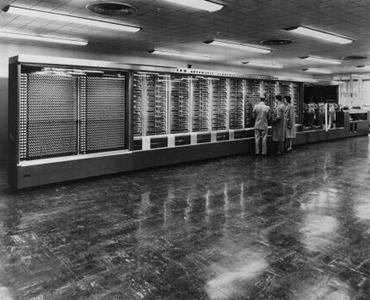
\includegraphics[width=.75\linewidth]{./Imagenes/ascc.jpg}}
			\caption{ASCC}
			\label{fig:ascc}
		\end{subfigure}%
		\begin{subfigure}{.5\textwidth}
			\centering
			\href{https://www-03.ibm.com/systems/z/hardware/z13.html}{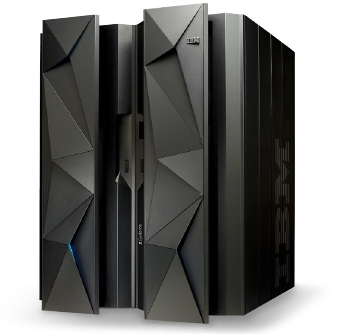
\includegraphics[width=.65\linewidth]{./Imagenes/z13.jpg}}
			\caption{\href{https://www-03.ibm.com/systems/z/}{Z13}}
			\label{fig:z13}
		\end{subfigure}
		\caption{Evolución mainframes}
	\end{figure}
\end{frame}

\begin{frame}{Posibles aplicaciones}
	\begin{figure}
		\centering
		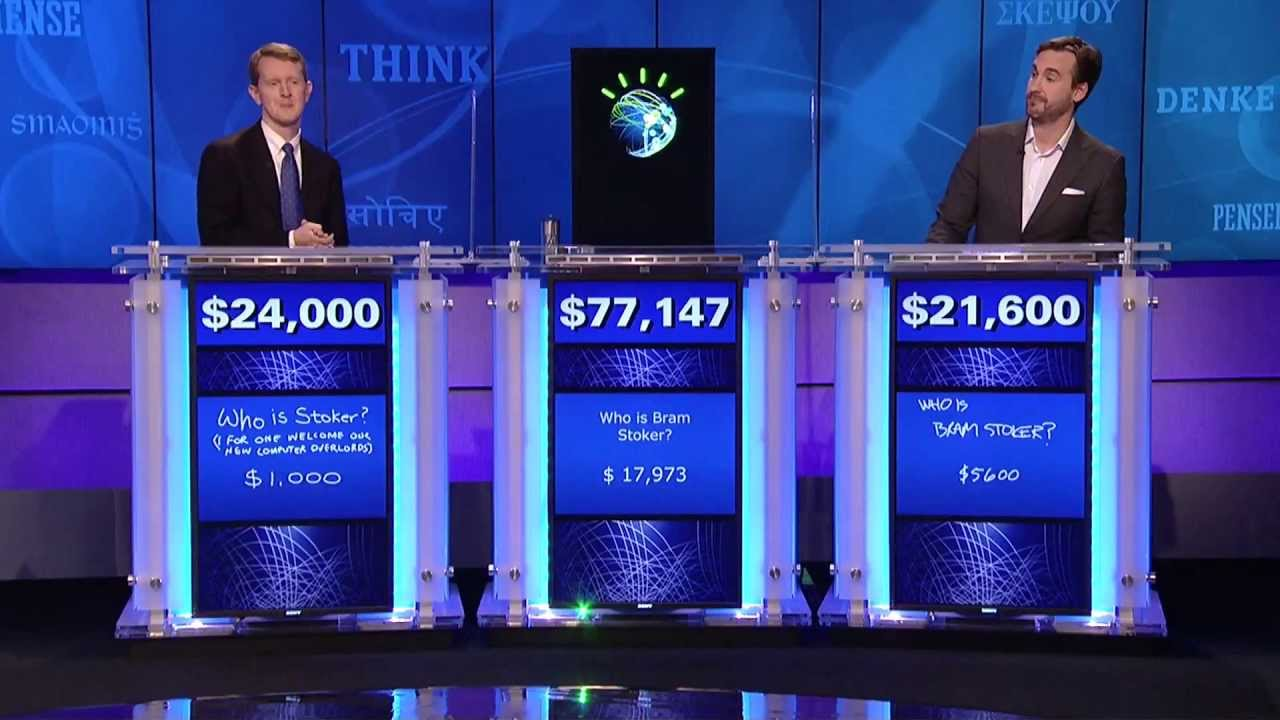
\includegraphics[width=.95\linewidth]{./Imagenes/j-watson.jpg}
		\caption{Watson en \textit{Jeopardy!}}
		\label{watson}
	\end{figure}
\end{frame}

\section{Mainframes}
\subsection{Evolución y características}
\begin{frame}
	\begin{block}{Grid computing}
		Uso descentralizado de diferentes recursos hardware y software
	\end{block}
	\begin{figure}
		\centering
		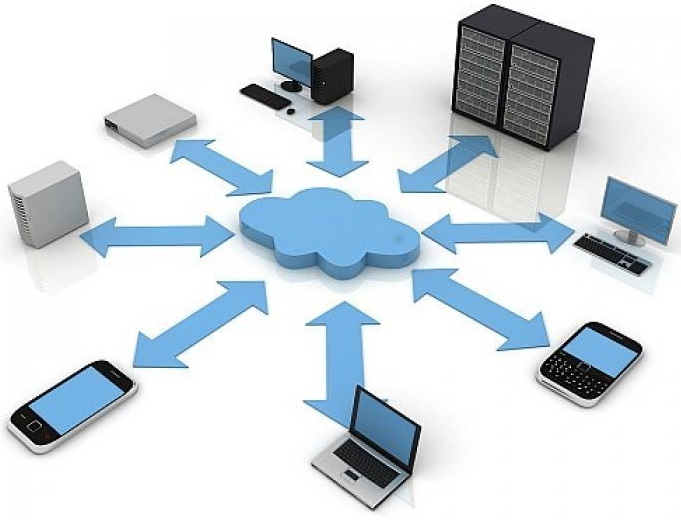
\includegraphics[width=.65\linewidth]{./Imagenes/grid-c.jpg}
		\caption{Grid computing}
		\label{grid-c}
	\end{figure}
\end{frame}


\begin{frame}
	\begin{exampleblock}{Términos}
		\begin{itemize}
			\item Servidor
			\item Granja
			\item Configuración dinámica
			\item Plataforma
		\end{itemize}
	\end{exampleblock}
	\begin{block}{Características mainframe}
		\begin{itemize}
			\item Altas prestaciones
			\item Seguridad
			\item Acceso a disco compartido
			\item Protección de los datos y control de privilegios
			\item Copias de seguridad y capacidad recuperación
			\item Varias copias del sistema operativo como un único sistema, o Parallel Sysplex (cluster en UNIX).
		\end{itemize}
	\end{block}
\end{frame}

\begin{frame}
	\begin{block}{Hardware}
		\begin{itemize}
			\item Procesadores
			\begin{itemize}
				\item Central Processor Complex
				\item System Assistance Processor (E/S)
				\item Integrated Facility for Linux (IFL)
				\item zAAP
				\item zIIP
				\item Integrated Coupling Facility
				\item Procesadores de respuesto: Spare
			\end{itemize}

			\item Disco SCSI
			
		\end{itemize}
	\end{block}
\end{frame}

\begin{frame}
	\begin{block}{Ventajas mainframe}
		\begin{itemize}
			\item El hardware tiene comprobación y recuperación de errores
			\item Reemplazamiento del hardware y el software
			\item Tipo de errores comprensible
		\end{itemize}
	\end{block}
	\begin{figure}[H]
		\centering
		\label{workloads}
		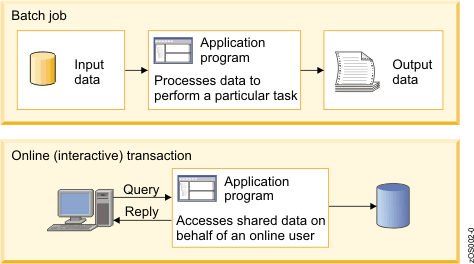
\includegraphics[trim = 0mm 0mm 5mm 0mm, clip, width=0.75\textwidth]{./Imagenes/workloads.png}
		\caption{Tipos de trabajo en un mainframe}
	\end{figure}
\end{frame}

\section{Watson}
\subsection{Características generales}
\begin{frame}{Watson}
	\begin{block}{Características Watson}
		\begin{itemize}
			\item Sistema QA (Question answering)
			\begin{itemize}
				\item Procesamiento
				de lenguaje natural (NLP)	
				\item Representación del conocimiento
				\item Razonamiento
			\end{itemize}
		\end{itemize}
	\end{block}
	\begin{block}{Características comunicación humana}
		\begin{itemize}
			\item Imperfección
			\item Polisemia
			\item Ironías
			\item Contexto
			\item Sin estructura
			\item Información implícita
		\end{itemize}
	\end{block}
\end{frame}

\subsection{Estructura}
\begin{frame}{Arquitectura Watson}
	\begin{block}{}
		La base de la arquitectura de Watson es UIMA (Unstructured Information Management Architecture), por encima se desarrolló DeepQA.
	\end{block}
	\begin{figure}[H]
		\centering
		\label{tiw-deepqa}
		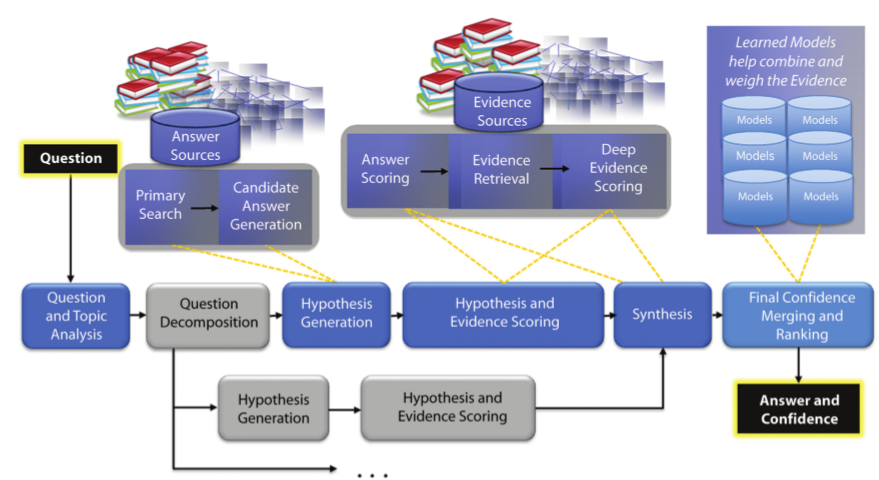
\includegraphics[width=0.8\textwidth]{./Imagenes/deepQA.png}
		\caption{Arquitectura DeepQA}
	\end{figure}
\end{frame}

\begin{frame}{Funcionamiento}
	\begin{block}{Entendiendo las preguntas}
		\begin{itemize}
			\item ESG (English Slot Grammar)
			\item Generador PAS (predicate-argument structure)
		\end{itemize}
		Para extraer conocimiento de
		las fuentes seleccionadas se usa PRISMATIC
	\end{block}
\end{frame}


\begin{frame}{Preguntas}
	\begin{exampleblock}{Tipo de respuesta (Dirección)}		
		Si usted está de pie, es la dirección que debe buscar para ver el revestimiento.
		
		Respuesta: Abajo
	\end{exampleblock}	

	\begin{exampleblock}{Relaciones (Madres e hijos)}
		Aunque solo les separa un año de vida, ella interpretó a la madre de Colin Farrell en Alexander.
		
		Respuesta: Angelina Jolie
		
		Relación: protagoniza(ella, Alexander)
	\end{exampleblock}
	
	\begin{exampleblock}{Consultas enlazadas}
		El nombre de este personaje, introducido en 1894, proviene de ”oso” en Hindi.
		
		Respuesta: Baloo
	\end{exampleblock}
\end{frame}

\begin{frame}{Evolución Watson}
	\begin{figure}[H]
		\centering
		\label{watson2today}
		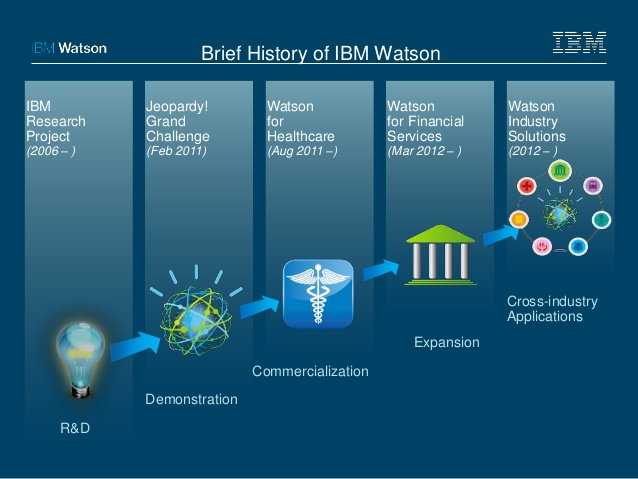
\includegraphics[trim = 0mm 14mm 0mm 10mm, clip, width=0.85\textwidth]{./Imagenes/watson2today.jpg}
		\caption{Evolución del sistema Watson}
	\end{figure}
\end{frame}

\section{IBM Bluemix}
\begin{frame}{IBM Bluemix}
	Plataforma de cloud computing que combina la plataforma como servicio
	(PaaS) con la infraestructura como servicio (IaaS).
	\begin{figure}[H]
		\centering
		\label{ibm-bluemix.jpg}
		
\includegraphics[width=0.45\textwidth]{./Imagenes/ibm-bluemix.jpg}
		\caption{Logo IBM Bluemix}
	\end{figure}

	\begin{exampleblock}{Posibilidades}
		\begin{itemize}
			\item Reconocimiento de lenguaje natural, emociones, imágenes, ...
			\item Traducción
			\item Conversión de formatos de archivo
			\item Agentes conversacionales
		\end{itemize}
	\end{exampleblock}
\end{frame}


\begin{frame}{Ejemplos}
	\begin{figure}[H]
		\centering
		\label{car1.jpg}
		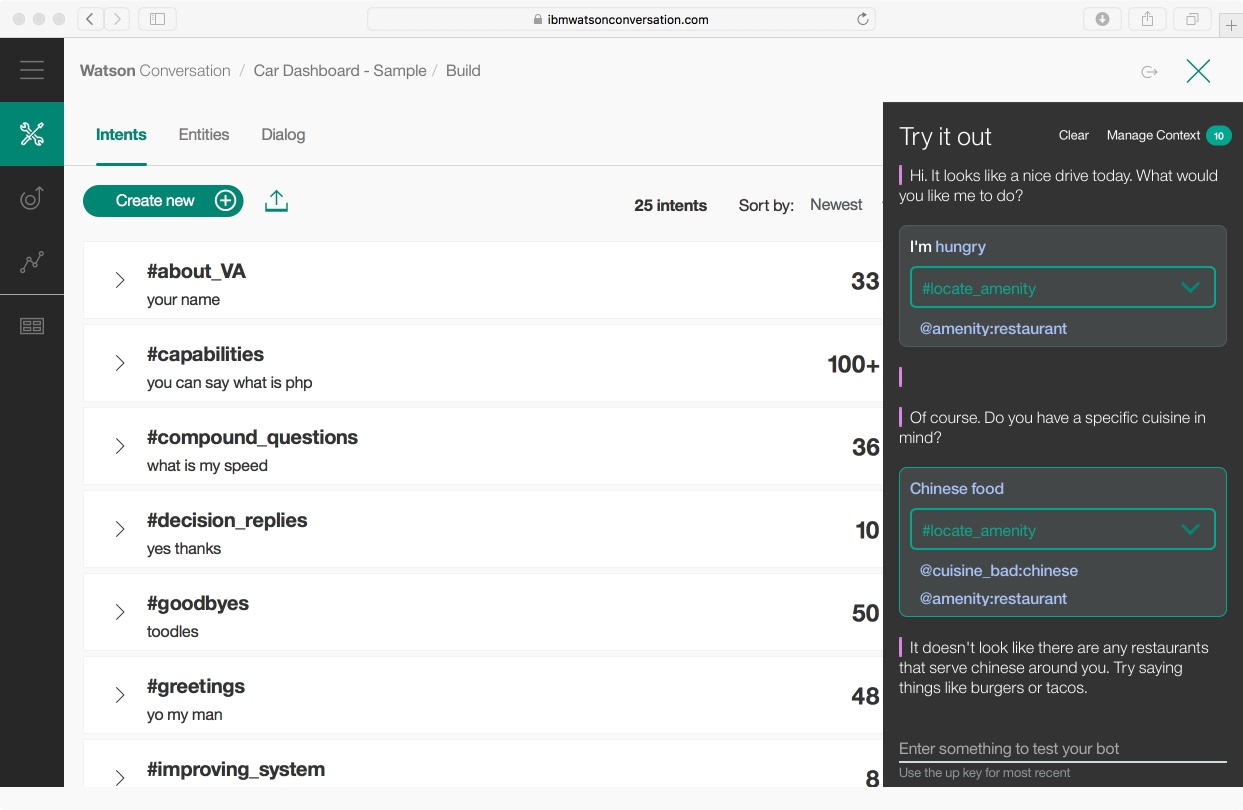
\includegraphics[width=0.99\textwidth]{./Imagenes/car1.jpeg}
		\caption{Agente conversacional para asistir en la conducción (1)}
	\end{figure}
\end{frame}

\begin{frame}
	\begin{figure}[H]
		\centering
		\label{car2.jpg}
		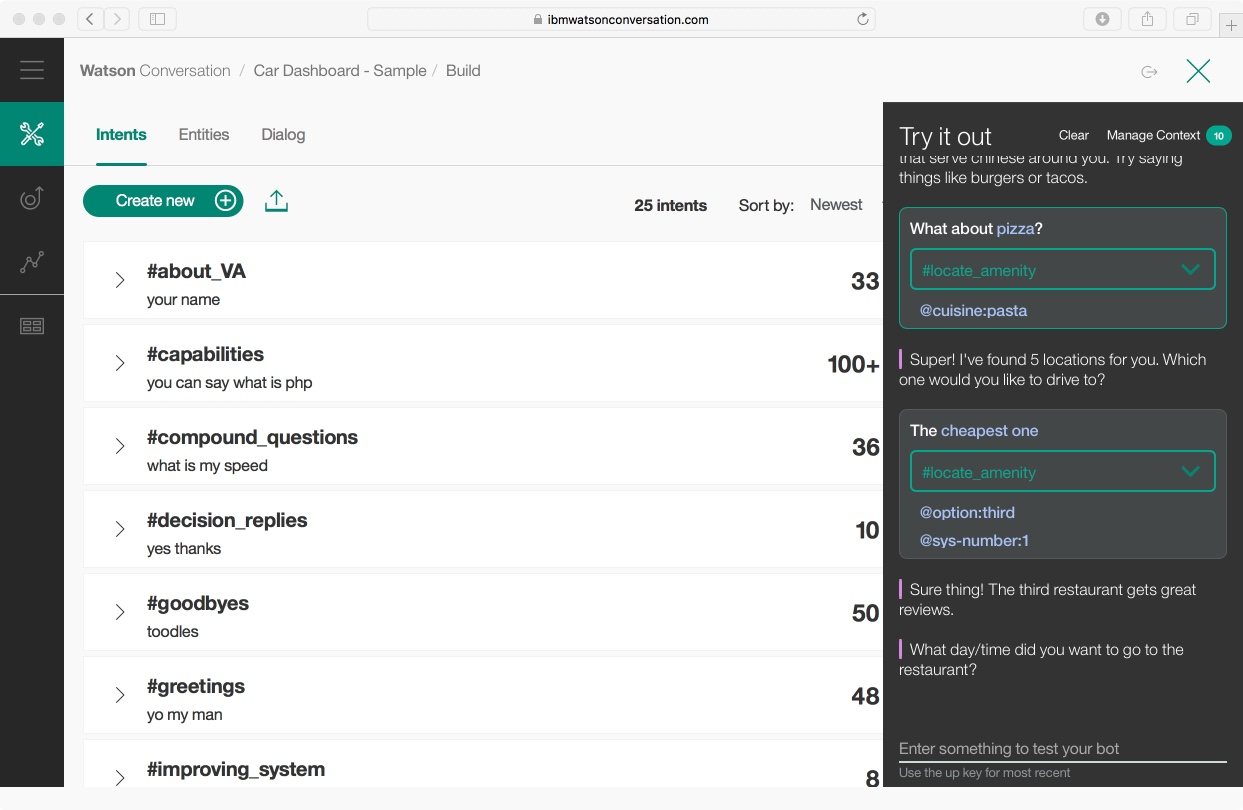
\includegraphics[width=0.99\textwidth]{./Imagenes/car2.jpeg}
		\caption{Agente conversacional para asistir en la conducción (2)}
	\end{figure}
\end{frame}

\begin{frame}
	\begin{figure}[H]
		\centering
		\label{anger.jpg}
		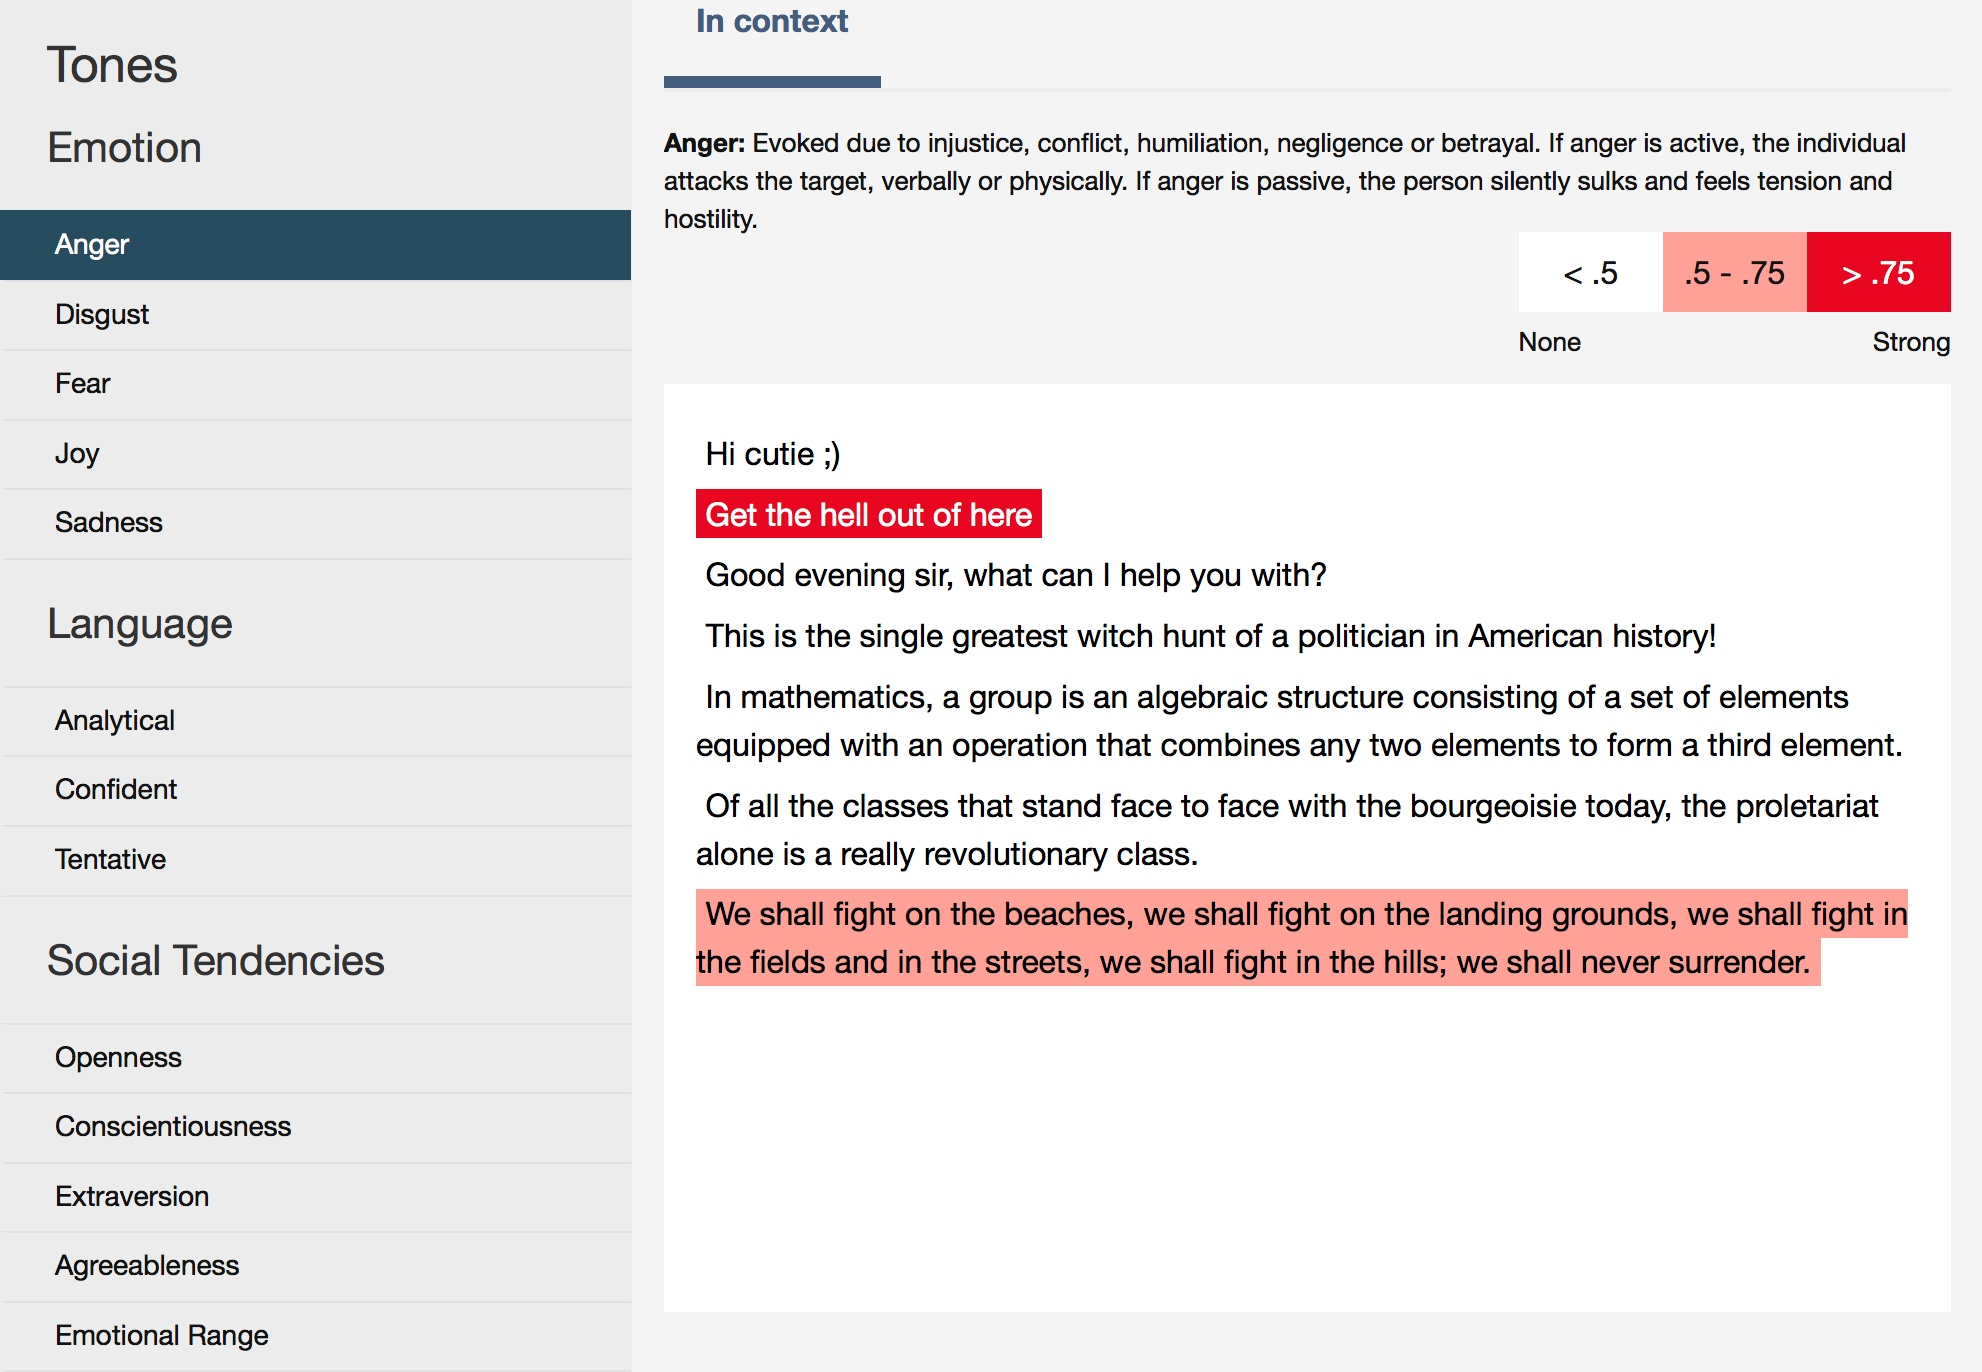
\includegraphics[width=0.99\textwidth]{./Imagenes/anger.jpeg}
		\caption{Ejemplo de detección de emociones (1)}
	\end{figure}
\end{frame}

\begin{frame}
	\begin{figure}[H]
		\centering
		\label{disgust.jpg}
		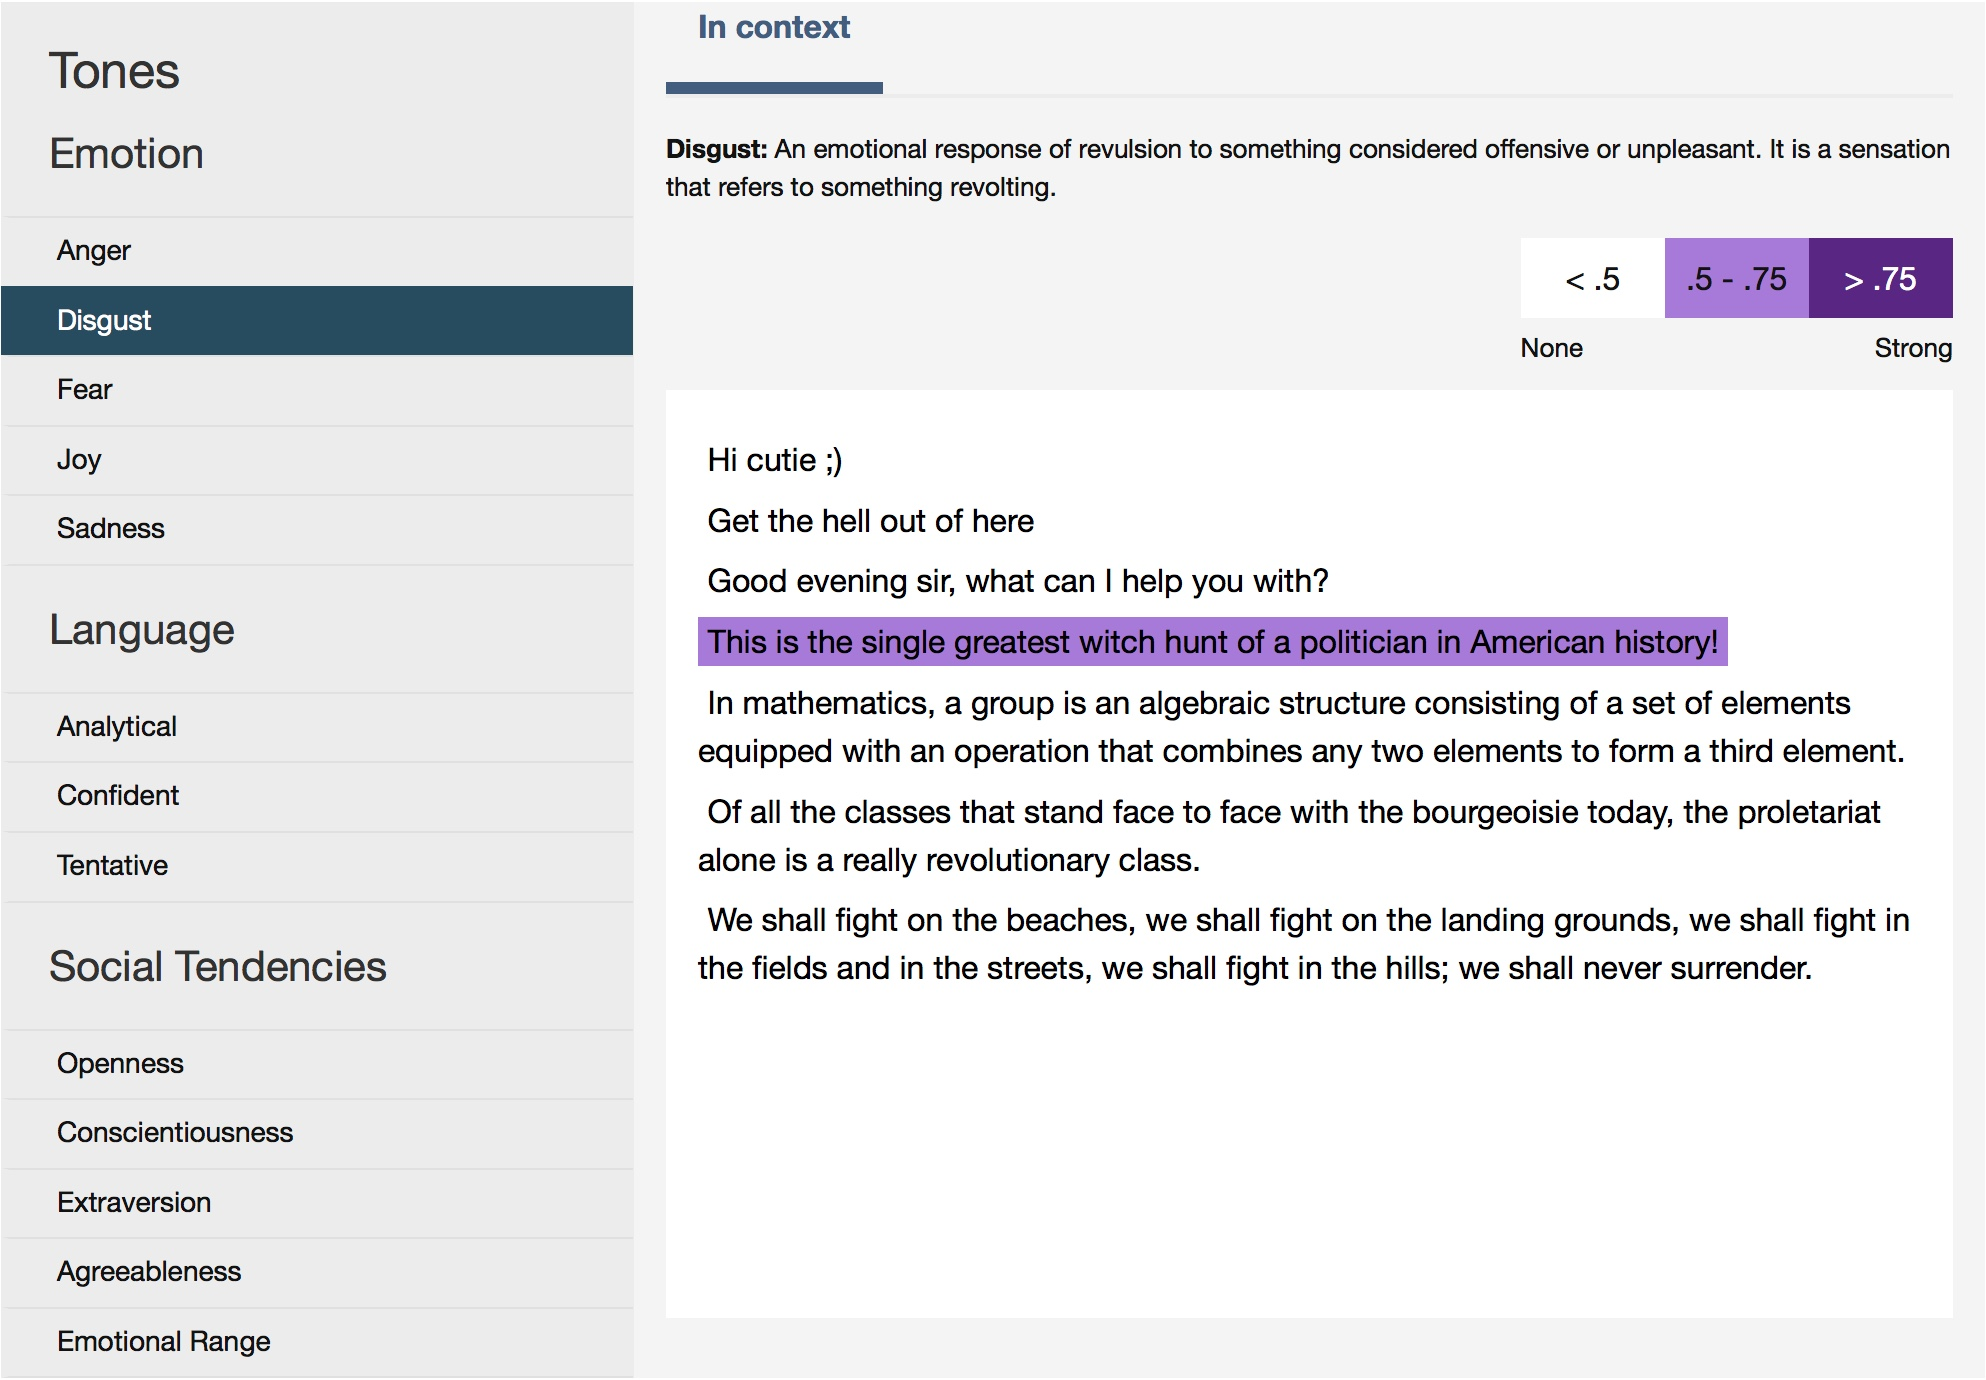
\includegraphics[width=0.99\textwidth]{./Imagenes/disgust.jpeg}
		\caption{Ejemplo de detección de emociones (2)}
	\end{figure}
\end{frame}

\begin{frame}
	\begin{figure}[H]
		\centering
		\label{sadness.jpg}
		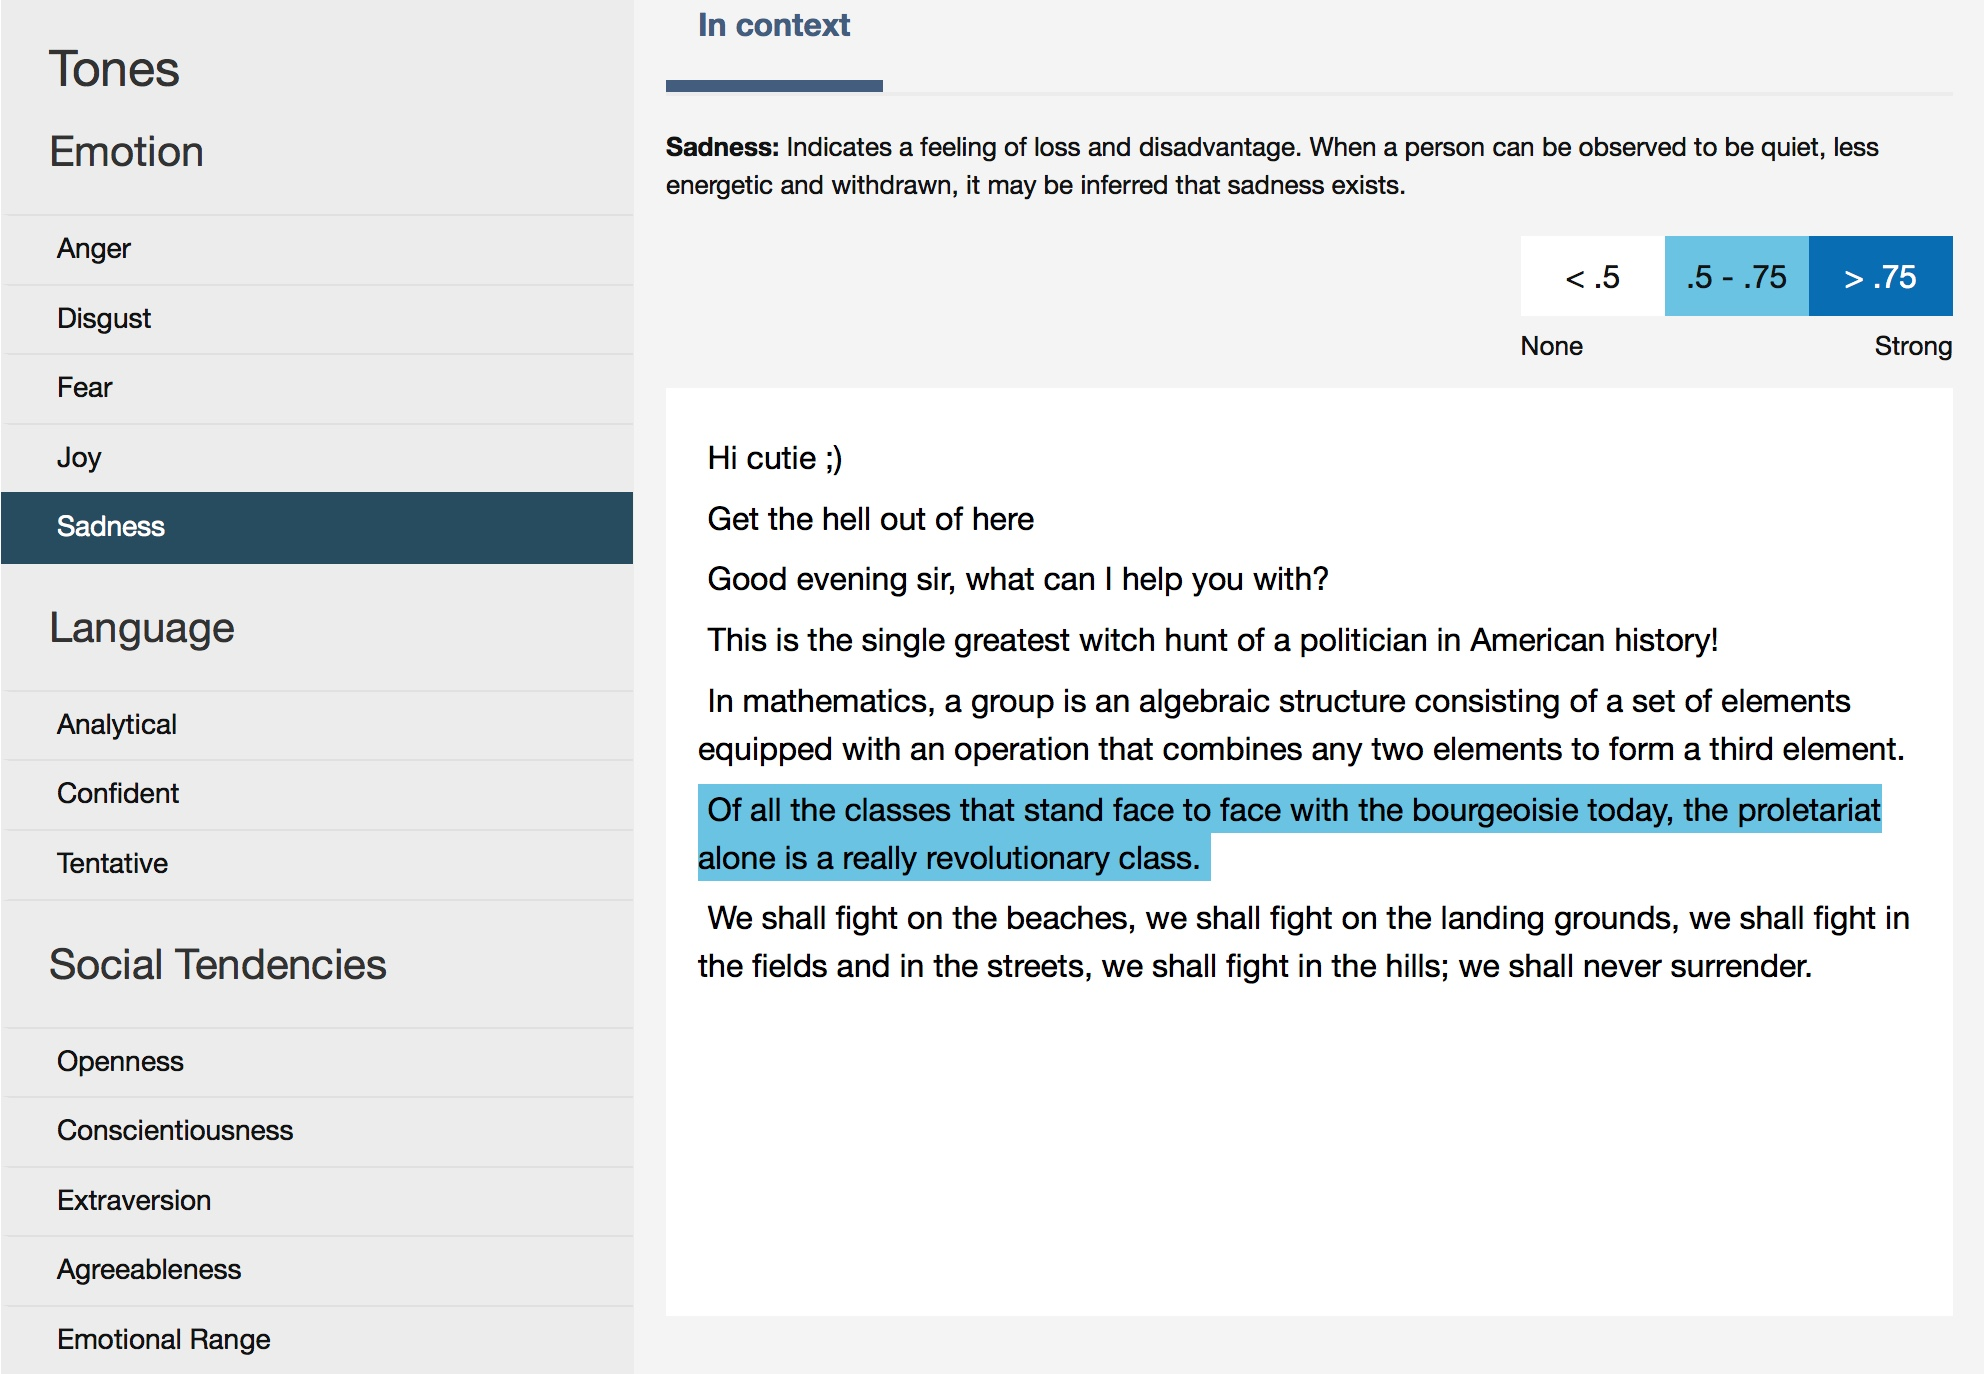
\includegraphics[width=0.99\textwidth]{./Imagenes/sadness.jpeg}
		\caption{Ejemplo de detección de emociones (3)}
	\end{figure}
\end{frame}

\begin{frame}
	\begin{figure}[H]
		\centering
		\begin{subfigure}{.5\textwidth}
			\centering
			\label{conversacion1.jpg}
			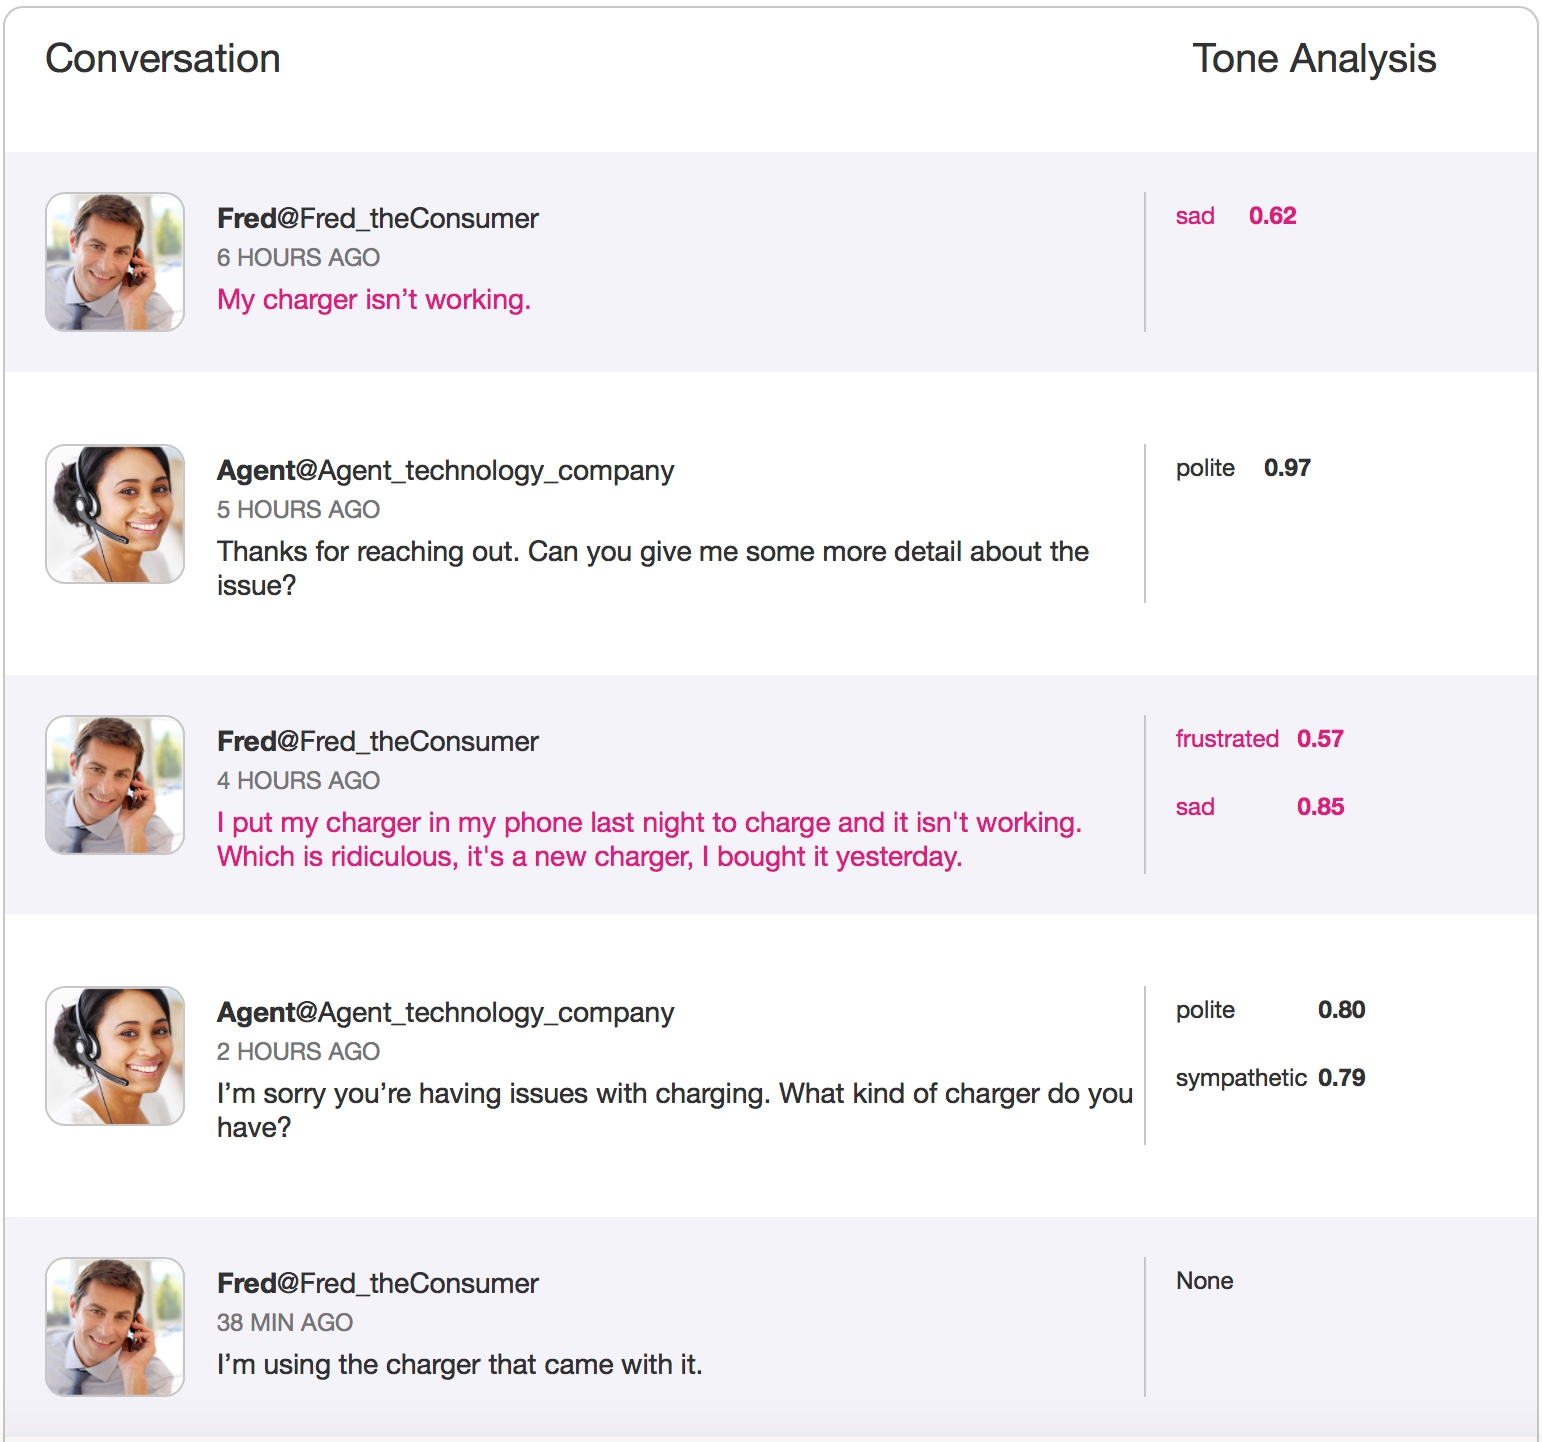
\includegraphics[width=0.99\textwidth]{./Imagenes/conversacion1.jpeg}
			\caption{Ejemplo de uso de detección de emociones para un serivicio técnico (1)}
		\end{subfigure}%
		\begin{subfigure}{.5\textwidth}
			\centering
			\label{conversacion2.jpg}
			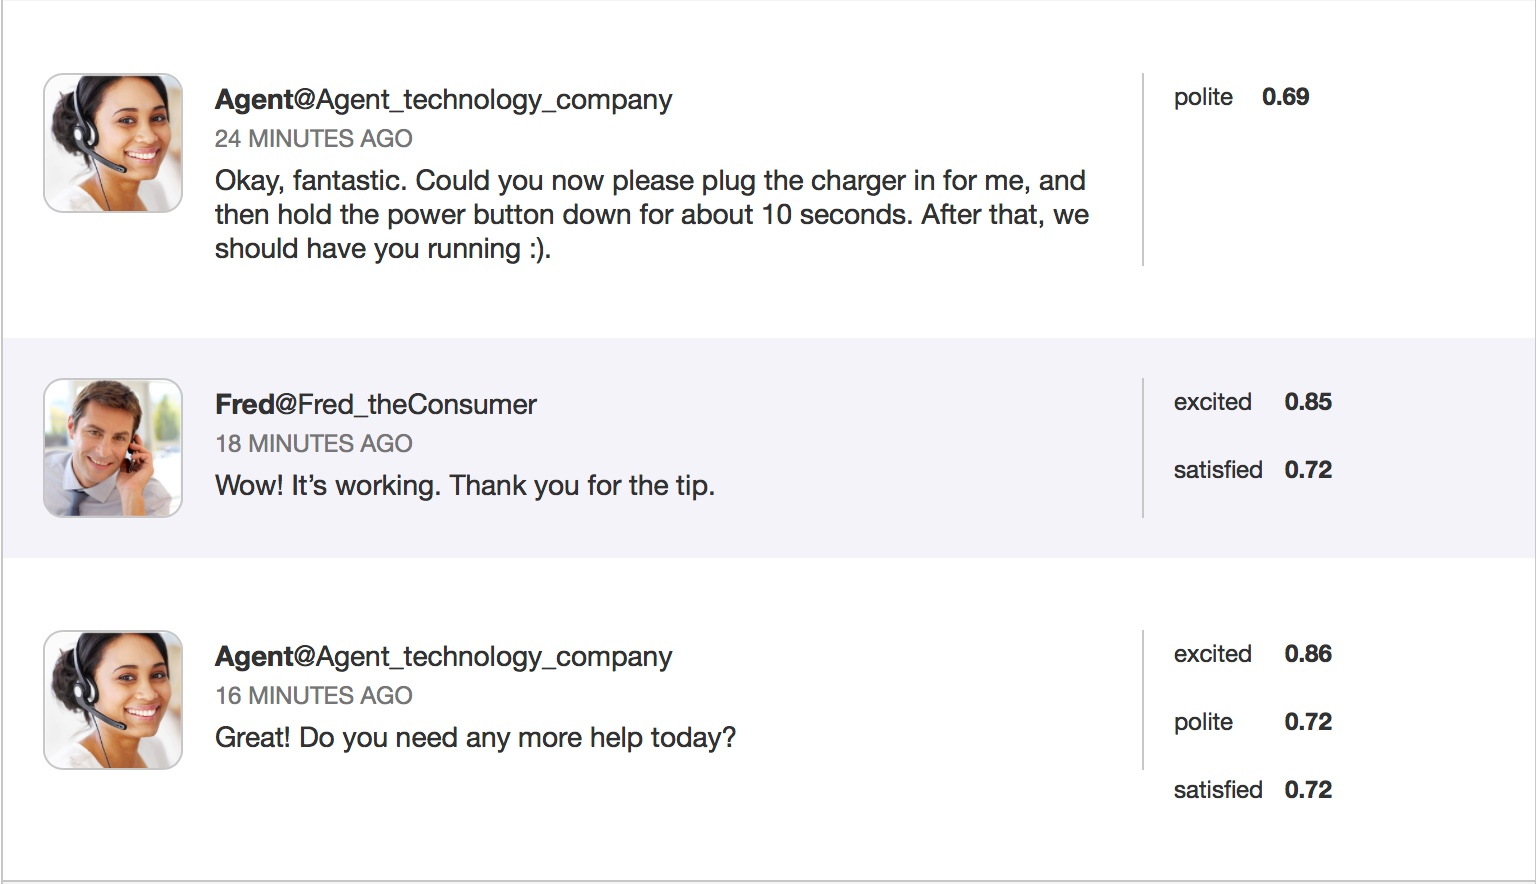
\includegraphics[width=0.99\textwidth]{./Imagenes/conversacion2.jpeg}
			\caption{Ejemplo de uso de detección de emociones para un serivicio técnico (2)}
		\end{subfigure}
	\end{figure}
\end{frame}

\begin{frame}{Conclusiones}
	
\end{frame}

\end{document}

